\section{Drift Chambers}\label{sec:clas.dc}

The \abbr{CLAS} drift chambers \abbr{DC} (Figs.~\ref{fig:clas},~\ref{fig:clas.dc.torus.cont},~\ref{fig:clas.dc.drift}) track charged particles above 200~MeV/c with polar angle resolution of 2-4~mrad and momentum resolution of 0.5 - 1\%, depending on momentum, see Fig~\ref{fig:clas.dc.res}. Typical coverage of the \abbr{DC} is $8^\circ < \theta < 142^\circ$, when the target is at \abbr{CLAS} center. For the \g12 experiment the coverage of the \abbr{DC} was modified to $6^\circ < \theta < 100^\circ$ due to the placement of the target, see Sec~\ref{sec:clas.tgt} for reasons explained in ~\cite{clas.proposal.hyclas},~\cite{clas.proposal.superg},~\cite{clas.proposal.pion}.
\begin{figure}\begin{center}
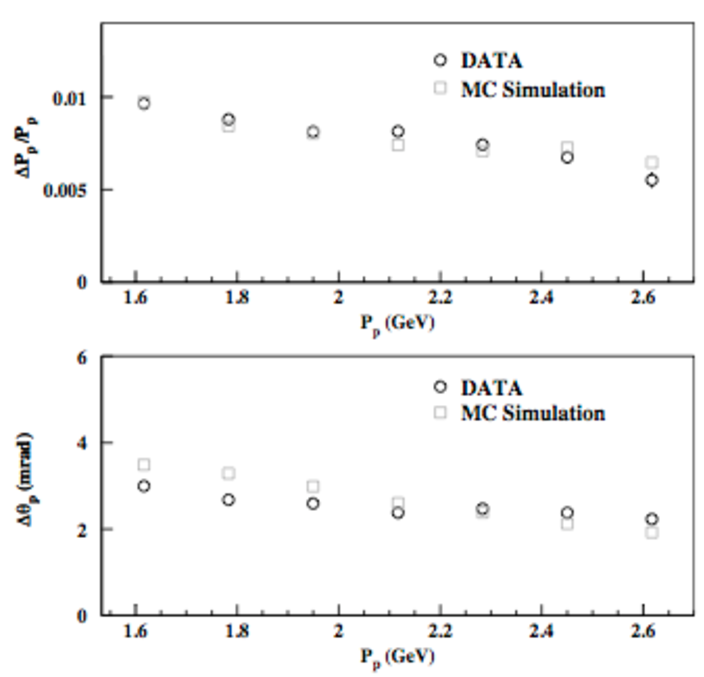
\includegraphics[width=0.8\figwidth,height=0.75\hfigheight]{\figures/hall-b/drift_DC_resolution.pdf}
\caption[Momentum and angular resolution for protons as determined from the measured angle of the scattered electron for data collected and Monte-Carlo simulation]{\label{fig:clas.dc.res}Momentum and angular resolution for protons as determined from the measured angle of the scattered electron for data collected and Monte-Carlo simulation. Image Source~\cite{clas}}
\end{center}\end{figure}

The \abbr{DC} are divided into six sectors each containing three radial layers (Fig.~\ref{fig:clas.dc.drift}), referred to as ``Regions'', for a total of 18 separate drift chambers. Each \abbr{DC} region covers the same polar angular range and consist of two superlayers which each contain six layers of hexagonal wire cells which house evenly spaced 20~$\mu$m gold-plated tungsten sense wires (center of hexagon) each surrounded by six 140~$\mu$m gold-plated aluminum alloy field wires (vertices of hexagon). In the first superlayer, the wires are strung approximately parallel to the direction of the magnetic field (axial wires), while the second superlayer has wires tilted at a 6$^\circ$ angle with respect to the axial wires (stereo wires). A high voltage system maintains the sense wires at positive potential, while the field wires are maintained at a negative potential 50\% lower than the positive value. The difference of potentials creates an avalanche of the electrons induced by the ionizing particle. The hexagonal shape of the cell mimics a circular geometry cell in which the drift time to drift distance is independent of entrance angle.

The inner region is denoted as Region 1. Its first superlayer has only 4 layers due to space constraints. Region 1 is nearly free from magnetic field, see Fig~\ref{fig:clas.dc.torus.mag}. Region 2 is situated between the magnetic coils which is subject to the highest magnetic field which is used to determine the particle's curvature, needed to determine the particle;s momenta, see Eq.~\ref{eq:motioninmag}. Region 3 purpose is to provide global track reconstruction in connection with other CLAS detectors since Region 3 is located outside the volume of magnetic field. Each \abbr{DC} is filled with a gas mixture of 90\% argon and 10\% carbon-dioxide. This choice of gas provides high drift velocity (0.04 m/$\mu$sec) and fast collection time which improves momentum resolution. For more information on the design of the \abbr{CLAS} \abbr{DC} system, see~\cite{clas.dc} and for more information on the calibration process of the \abbr{CLAS} \abbr{DC} system, see~\cite{clas.dc.calib}.

\begin{figure}\begin{center}
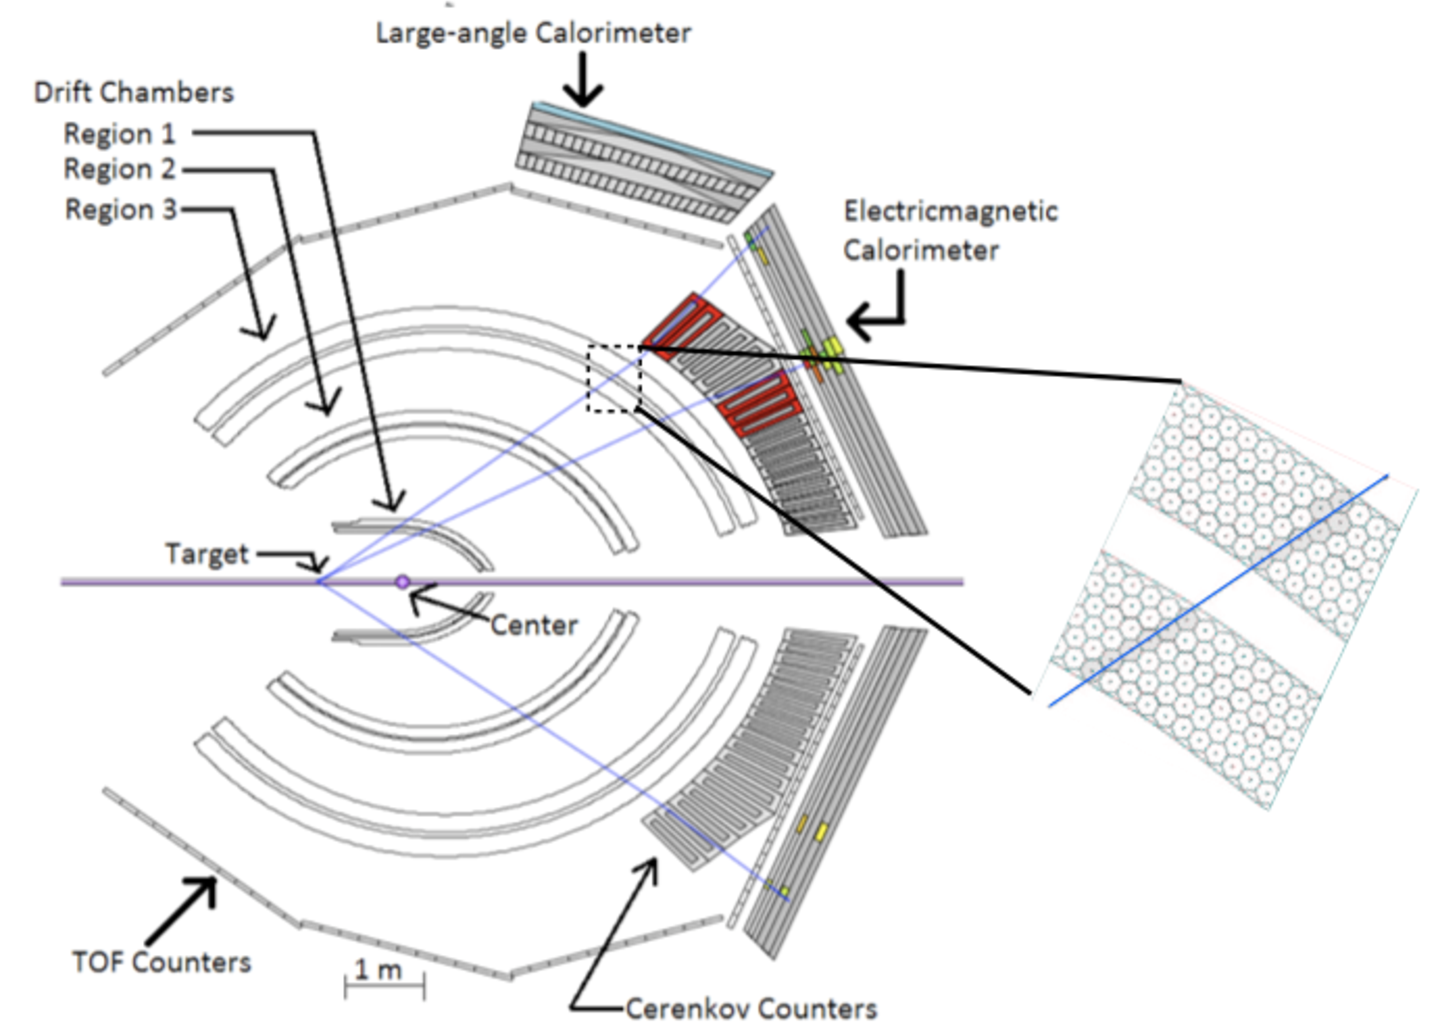
\includegraphics[width=\figwidth,height=0.75\hfigheight]{\figures/hall-b/drift_DC_cedII.pdf}
\caption[A cross section view of the \abbr{CLAS} detector showing an event with three tracks emanating from the target]{\label{fig:clas.dc.drift}A cross section view of the \abbr{CLAS} detector showing an event with three tracks emanating from the target. The two tracks leaving hit patterns \abbr{CC} and \abbr{EC} are leptons while the track on the bottom panel is a proton. The inlet shows hexagonal cells of drift chambers with a typical track indicated by shaded areas for the cut-out in Region-3.}
\end{center}\end{figure}
